\section{Optimality}
We claim that the symmetry elimination procedure outlined earlier is sufficient to 
guarantee that A*, running on our pruned grid maps, will always return an optimal solution if one exists.

\begin{theorem}
\label{thm-optimality}
For every optimal length path $\pi^*(s, g)$ in a 4-connected grid map there exists
an equivalent length path in the pruned version of the grid map.
\end{theorem}
\begin{proof}
Follows from Lemma \ref{thm-roomtraversal} and Lemma \ref{thm-insertion}.
For every optimal length segment of $\pi^{*}(s, g)$ which traverses
through an empty room, from a perimeter node $m$ to a perimeter node $n$, 
there is an equivalent segment which mentions only nodes
on the perimeter of that room (and possibly one macro-step).
\end{proof}

A direct corollary of Theorem \ref{thm-optimality} is that optimal solutions
pruned by our symmetry reduction can be easily reconstructed; for example to
avoid unnatural looking paths where agents seem to hug walls.
Consider a path fragment between $m$ and $n$, two nodes on the perimeter of an empty room.
Assume, without any generality loss, that the path fragment contains $r$ moves to the right and $u$ moves upwards.
All optimal path fragments between $m$ and $n$ can be obtained by interleaving $r$ moves to the right
and $u$ moves upwards in any order (e.g right-right-up, up-right-up, up-right-right)


\begin{figure}[t]
%	\vspace{-4pt}
\centering
	    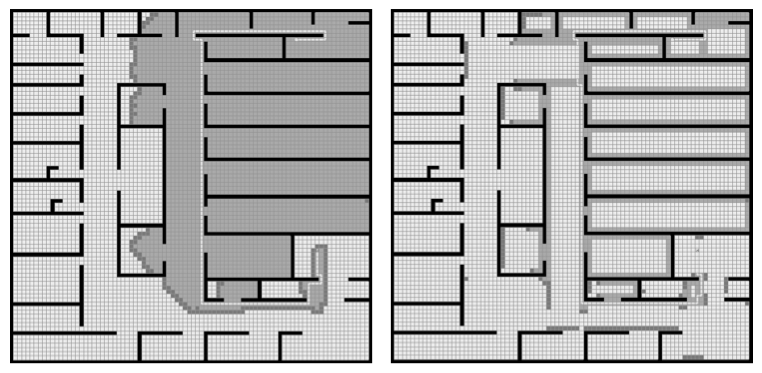
\includegraphics[width=0.95\columnwidth, trim = 10mm 10mm 10mm 0mm]{diagrams/oha_contrast.png}
		\caption{(Left) A* solving a problem on an unmodified ($86\times88$) grid map. 
		Expanded nodes are marked dark grey.
		(Right) A* solving the same problem using our modified grid map. 
		The algorithm only considers nodes along the perimeter of the identified rooms.}
	\label{fig-contrast}
\end{figure}

In Figure \ref{fig-contrast} we highlight the effectiveness of our symmetry breaking technique using
a map that has characteristics typical of what one might expect in a modern role-playing game\footnote{
In fact, many video game maps tend to be somewhat bigger than our example but for demonstration 
purposes it is sufficient.};
there are many rooms and corridors and many entrances connecting them.
A* running on the original grid map expands almost half the nodes
in the state space of the shown example.
We then apply our technique to eliminate symmetries and re-run A*.
This time A* expands less than 15\% of all nodes (more than a three-fold
improvement) and returns an optimal solution 3 times faster.
